\documentclass[11pt,letter]{article}
\usepackage[utf8]{inputenc}
\usepackage{amsmath}
\usepackage{amsfonts}
\usepackage{wrapfig}
\usepackage{amssymb}
\usepackage{graphicx}
\usepackage{hyperref}
\usepackage[left=3cm,right=3cm,top=3cm,bottom=2cm]{geometry}
\begin{document}
\pagestyle{empty}
\noindent
\begin{wrapfigure}{r}{0.25\textwidth}
    \centering
    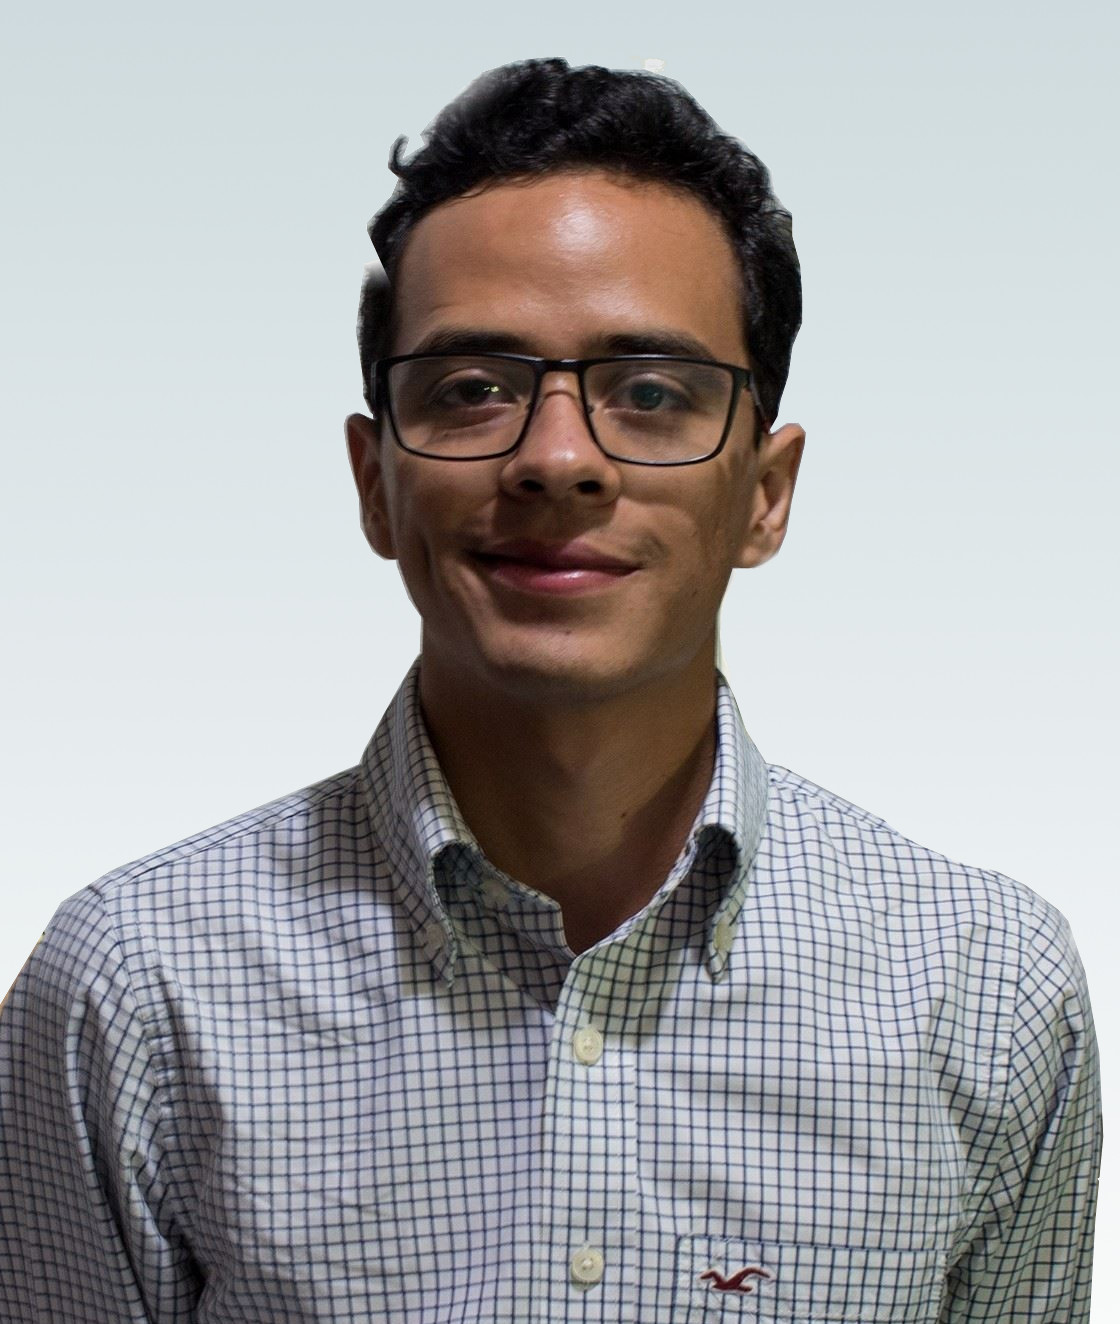
\includegraphics[width=0.2\textwidth]{CV}
\end{wrapfigure} 
\Large{\textbf{Alejandro López Hernández}}  
\\
\normalsize
Villa Federal Mz 13 Lt 6\\ Col. Hank Gonzalez, C.P. 09700, \\Izatapalapa, Ciudad de México, México\\ email: \href{mailto:aleespazx@gmail.com}{aleespazx@gmail.com}\\Tel: 55 40385923 \\ Fecha de Nacimiento 04/02/1996 (22 años)\\ Blog personal: \url{http://cienciactuarial.blogspot.mx/}\\\\
\noindent
\textbf{Resumen}\\
Estudiante de alto rendimiento en la licenciatura en actuaría que esta interesado en resolver problemas del mundo real utilizando como herramienta la estadística y la probabilidad en conjunto con mis habilidades de programación. Mi principal motivación es poder encontrar solución a problemas que son de gran impacto en la sociedad. \\
\textbf{Educación}\\
(2014 - Presente) 8vo semestre de Actuaría en la Facultad De Estudios Superiores Acatlán (UNAM) con promedio de 9.65\\\\
\textbf{Experiencia Laboral}\\
(2016 - 2017) \quad Ayudante de profesor en las asignaturas de Álgebra Lineal I y Álgebra Lineal II\\\\
\textbf{Idiomas}
\begin{itemize}
\item Ingles fluido
\end{itemize}
\textbf{Habilidades}
\begin{itemize}
\item Programación en Python intermedia
\item Programación en R básica
\item Manejo MS Office Excel
\item Manejo de SQL básico
\end{itemize}
\textbf{Actividades Académicas}
\begin{itemize}
\item 2017 - Tome el curso "Proyecta 10 000 Study Tour" impartido por MacEwan University en la ciudad de Edmonton, AB, Canada.
\item 2017 - Curso de creación de documentos LaTeX
\item 2016 - Asistí al 4to coloquio de estadística, organizado por la división de matemáticas e ingeniería de la FES Acatlán.
\item 2015 - Participé en el simulador bursátil, organizado por la FES Acatlán como motivo de su 40 aniversario.
\item 2014 - Gane el concurso "Let's Go to San Antonio", y tome un curso de ingles en la ciudad de San Antonio, TX, USA. 
\end{itemize}
\end{document}